\title{Consideration of spatial response functions when converting L2 data to L3}

\author{Kang Sun}
\documentclass[hidelinks,12pt]{article}
\usepackage{amsmath}
\usepackage[letterpaper,left=.75in,right=.75in,top=.75in,bottom=.75in]{geometry}
\usepackage{setspace}
\usepackage{lineno}
\newcommand{\beginsupplement}{%
        \setcounter{table}{0}
        \renewcommand{\thetable}{S\arabic{table}}%
        \setcounter{figure}{0}
        \renewcommand{\thefigure}{S\arabic{figure}}%
     }
\usepackage[section]{placeins}
\usepackage{subfig}
\usepackage{threeparttable,booktabs}
\usepackage[square]{natbib}
\usepackage{longtable}
\usepackage{multirow}
\usepackage{graphicx}
\usepackage[space]{grffile}
\usepackage{color}
\usepackage{hyperref}
\hypersetup{%
    pdfborder = {0 0 0}
}
%\usepackage{etoolbox}
\usepackage{gensymb}
%\usepackage{subcaption}
%\appto\TPTnoteSettings{\footnotesize}


\begin{document}
\maketitle
\abstract
This report documents the effort to incorporate spatial response function into the tessellation algorithm, which averages L2 satellite pixels into a L3 latitude-longitude grid. The tessellation code originated from Kai Yang and Lei Zhu.

\section{The ``cake cut'' method}

\begin{figure}[hbtp]
 \centering
 \subfloat{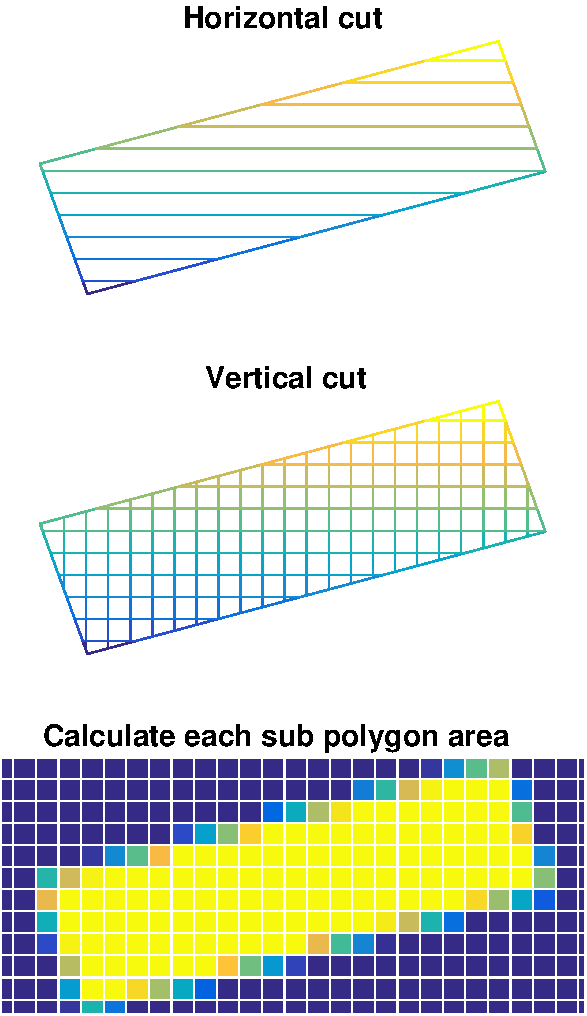
\includegraphics[width=.3\linewidth]{../plot/omi_pixel.pdf}}
 \quad \quad
\subfloat{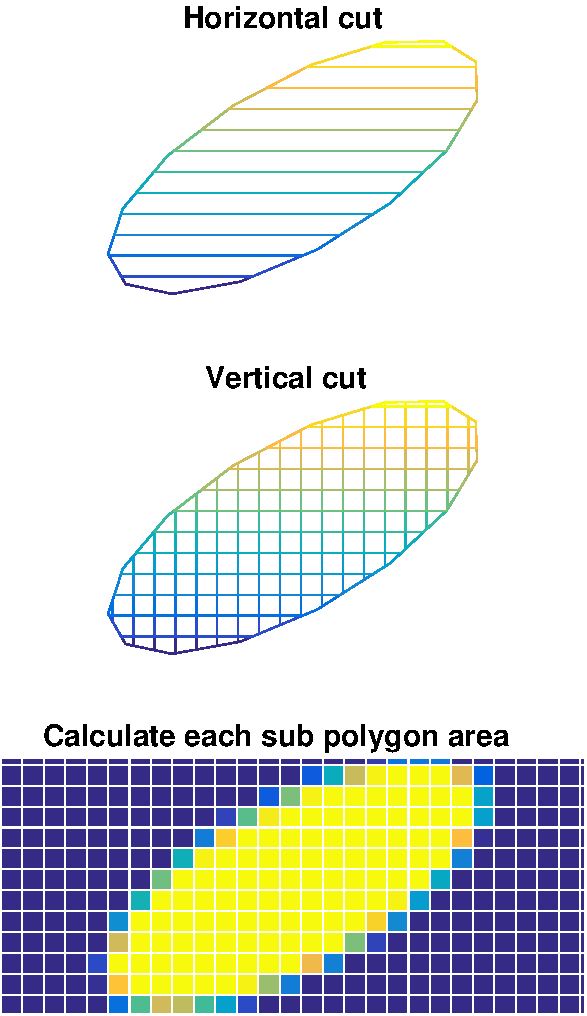
\includegraphics[width=.3\linewidth]{../plot/ellipse_pixel.pdf}}  \caption{Illustration of Kai Yang's cake cut program. The left is an OMI pixel. The right is an arbitrary elliptical polygon.}
    \label{fig1}
\end{figure}
\FloatBarrier
The cake cut method includes two basic functions. One cuts an arbitrary polygon horizontally at a certain resolution; the other one cuts an arbitrary polygon vertically. First cutting the L2 pixel horizontally, and then cutting each horizontal sub pixels vertically maps the polygon onto the tessellated grid. In my current Matlab implementation, the area of the fraction of the polygon in each tessellated grid is calculated by the built-in ``polyarea'' function, if the grid is not a square (i.e., on the boundary of L2 pixel). The grid areas inside the L2 pixel is just the square of the resolution.

\section{Spatial response functions (SRF)}
\begin{figure}[hbtp]
 \centering
 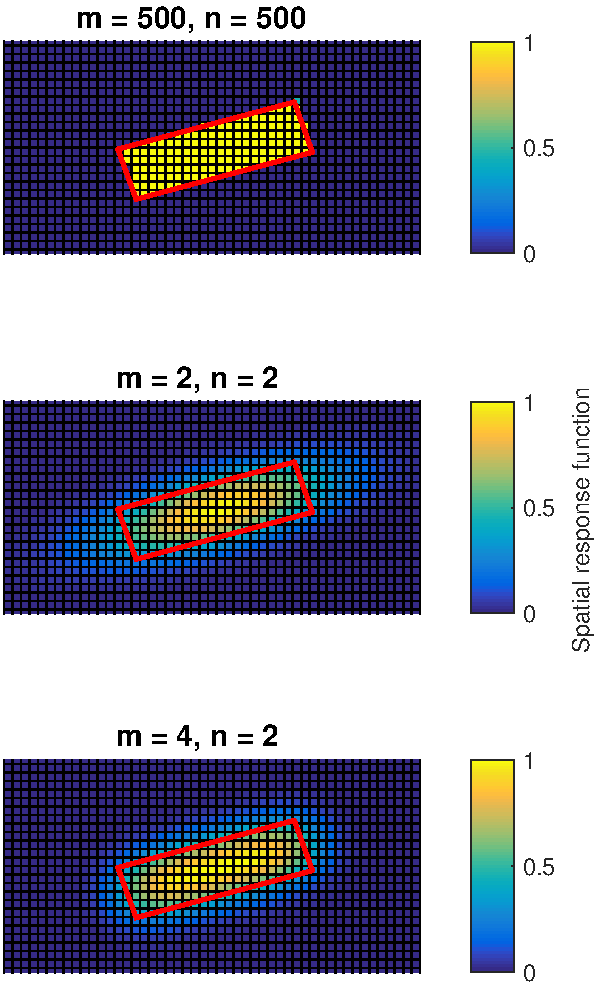
\includegraphics[width=.5\linewidth]{../plot/spatial_response.pdf}
 \caption{Spatial response function parameterized by 2-D super Gaussian functions. The red box is an OMI pixel.}
 \label{fig2}
 \end{figure}

The basic tessellation does not consider the spatial response function of L2 pixels. Namely the response is assumed to be 100 \% within the pixel boundary and zero outside. \citet{graaf2016how} characterized the spatial functions of OMI pixels at different cross-track positions and parameterized them by two-dimensional super Gaussian function (see Fig.~\ref{fig2} for 2-D super Gaussian of different exponents and Fig.~\ref{fig3} for the exponents measured for OMI pixels):

\begin{equation*}
g(x,y) = \exp \left( -\left( \frac{x}{w_x}\right)^m -\left( \frac{y}{w_y}\right)^n\right),
\end{equation*}
where
\begin{align*}
w_x & = \frac{\text{FWHM}_x}{2(\ln 2)^{1/m}};\\
w_y & = \frac{\text{FWHM}_y}{2(\ln 2)^{1/n}}.
\end{align*}
FWHM$_x$ and FWHM$_y$ are the cross-track and along-track widths of OMI L2 pixel, approximated by a rectangle.
 \begin{figure}[hbtp]
 \centering
 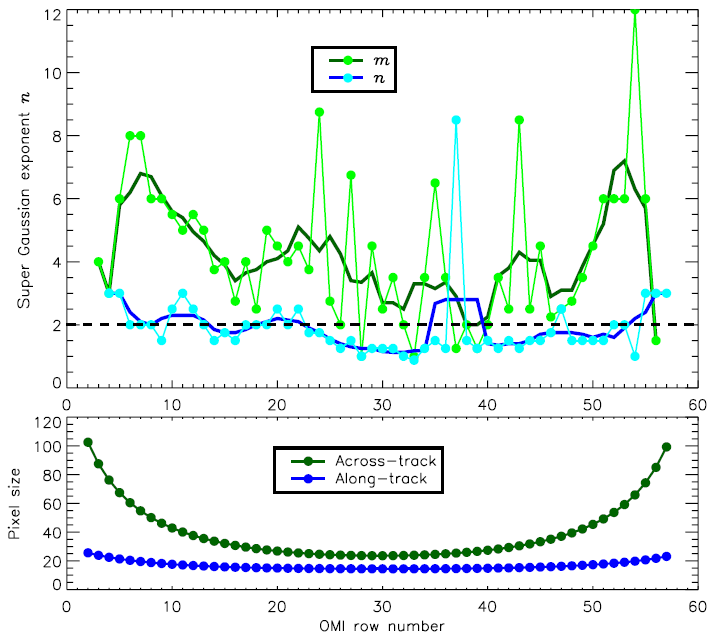
\includegraphics[width=.5\linewidth]{../plot/amt_fig9.png}
 \caption{OMI spatial response function exponents measured by \citet{graaf2016how}.}
 \label{fig3}
 \end{figure}

\section{Incorporation of SRF into the tessellation}
The SRF goes beyond the traditional boundary of an OMI pixel, so it is necessary to tessellate a larger area. As shown by Fig.~\ref{fig3}, the OMI SRF exponents are $\sim2$ in the along track direction and $\sim4$ in the cross-track direction. To include areas with significant SRF contribution, the OMI pixel is ``inflated'' by a factor of 1.5 across track and 2 along track. The tessellation algorithm is applied to the inflated OMI pixel instead. Then the total weight is the product of the area of the sub polygon in each grid cell and the SRF of each grid cell.

Because the SRF is small at the boundary of the inflated OMI pixel, the area of these sub polygons are not as important. The boundary of the inflated OMI pixel is somewhat arbitrary anyway. The right columns of Fig.~\ref{fig4} and Fig.~\ref{fig5} show simplified area calculation; for all grid cells overlaping the OMI pixel, the area of associated sub polygon is the square of the resolution. This simplification has little impact on the total weight for high resolution oversampling (compare Fig.~\ref{fig5} with Fig.~\ref{fig4}).

\begin{figure}[hbtp]
 \centering
 \subfloat{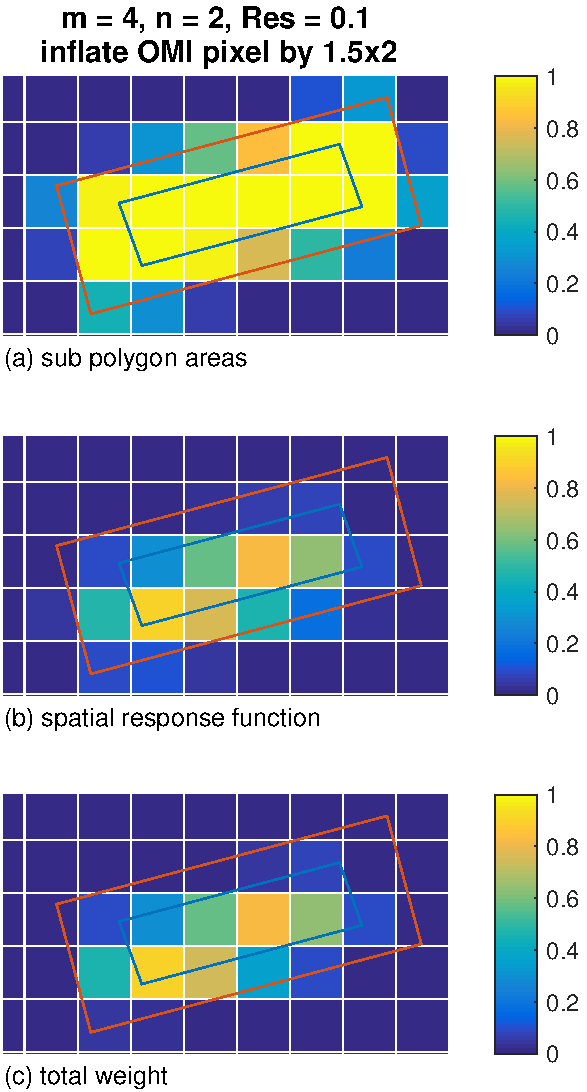
\includegraphics[width=.4\linewidth]{../plot/SRF_weight_inflate_1.5_2_Res_0.1_simplearea_0.pdf}}
 \quad \quad
\subfloat{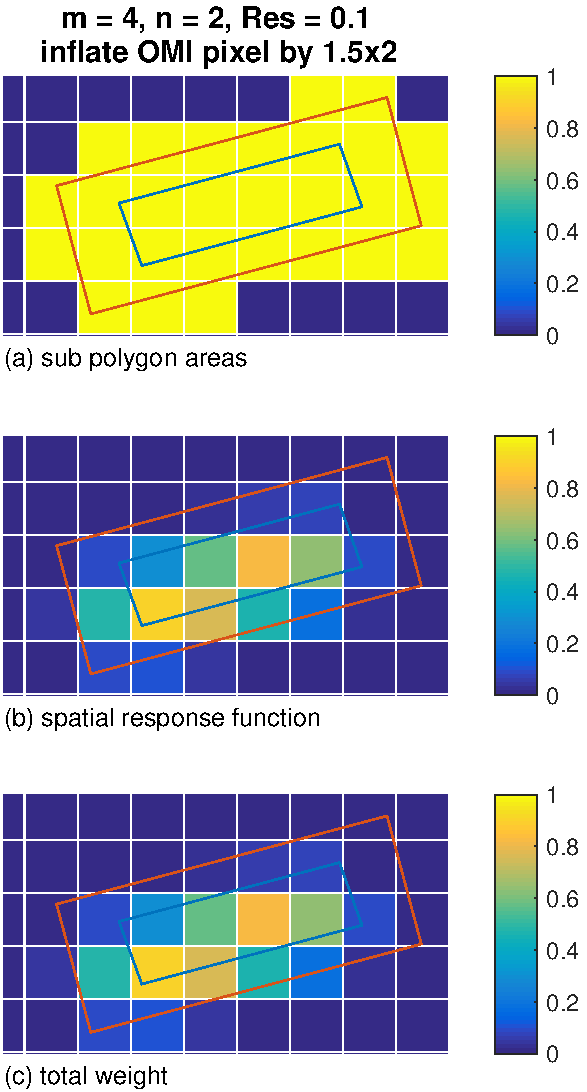
\includegraphics[width=.4\linewidth]{../plot/SRF_weight_inflate_1.5_2_Res_0.1_simplearea_1.pdf}}  \caption{Left: tessellated sub polygon areas (top), SRF values associated with each grid cell (middle), and the product of the two (bottom). The blue box is the original OMI pixel, and the red box is the inflated OMI pixel. Right: similar to the right but the sub polygons are all simplified as squares.}
    \label{fig4}
\end{figure}

\begin{figure}[hbtp]
 \centering
 \subfloat{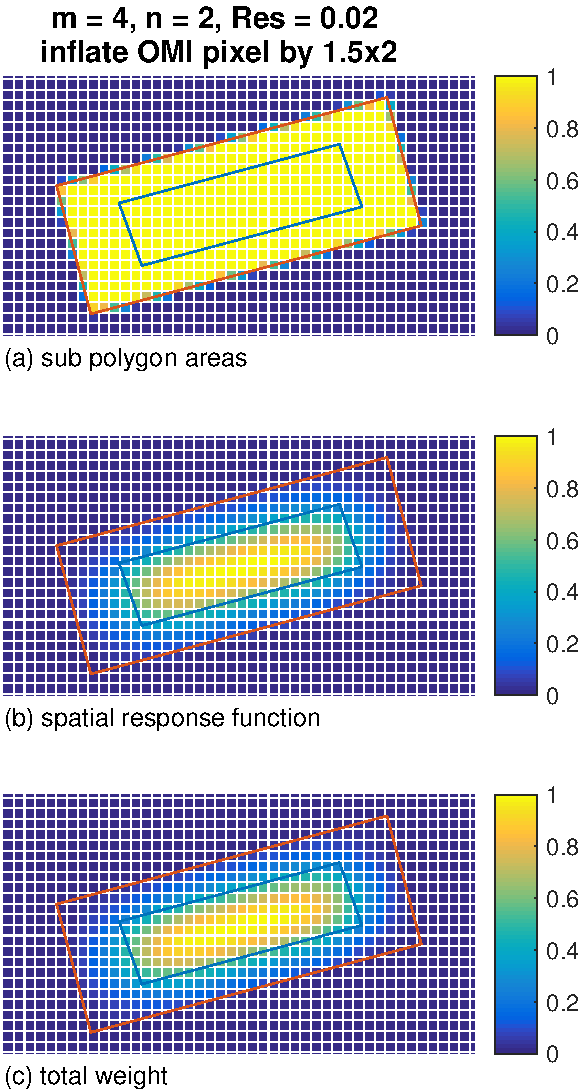
\includegraphics[width=.4\linewidth]{../plot/SRF_weight_inflate_1.5_2_Res_0.02_simplearea_0.pdf}}
 \quad \quad
\subfloat{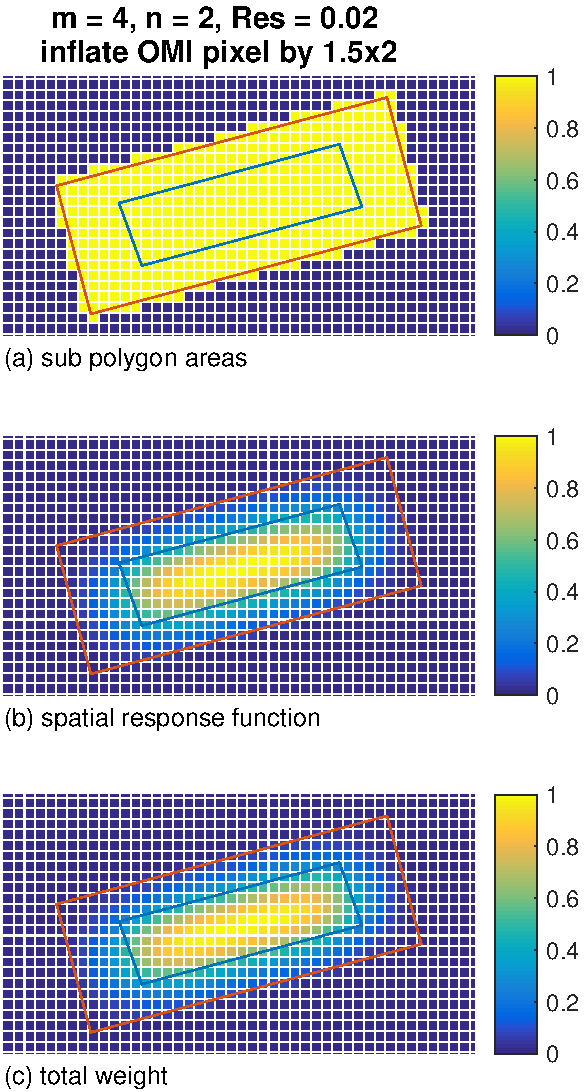
\includegraphics[width=.4\linewidth]{../plot/SRF_weight_inflate_1.5_2_Res_0.02_simplearea_1.pdf}}  \caption{Same as Fig.~\ref{fig4} but at higher resolution (0.02 instead of 0.1 degree).}
    \label{fig5}
\end{figure}

\FloatBarrier

\section{L3 results}
Figure~\ref{fig6} compares the L3 map of HCHO oversampled using basic tessellation and different assumptions of SRF. When the 2-D super Gaussian exponents are large, it approximates to the basic tessellation. Smaller exponents mean more spread SRF and smoother oversampled L3 map.

\begin{figure}[hbtp]
 \centering
 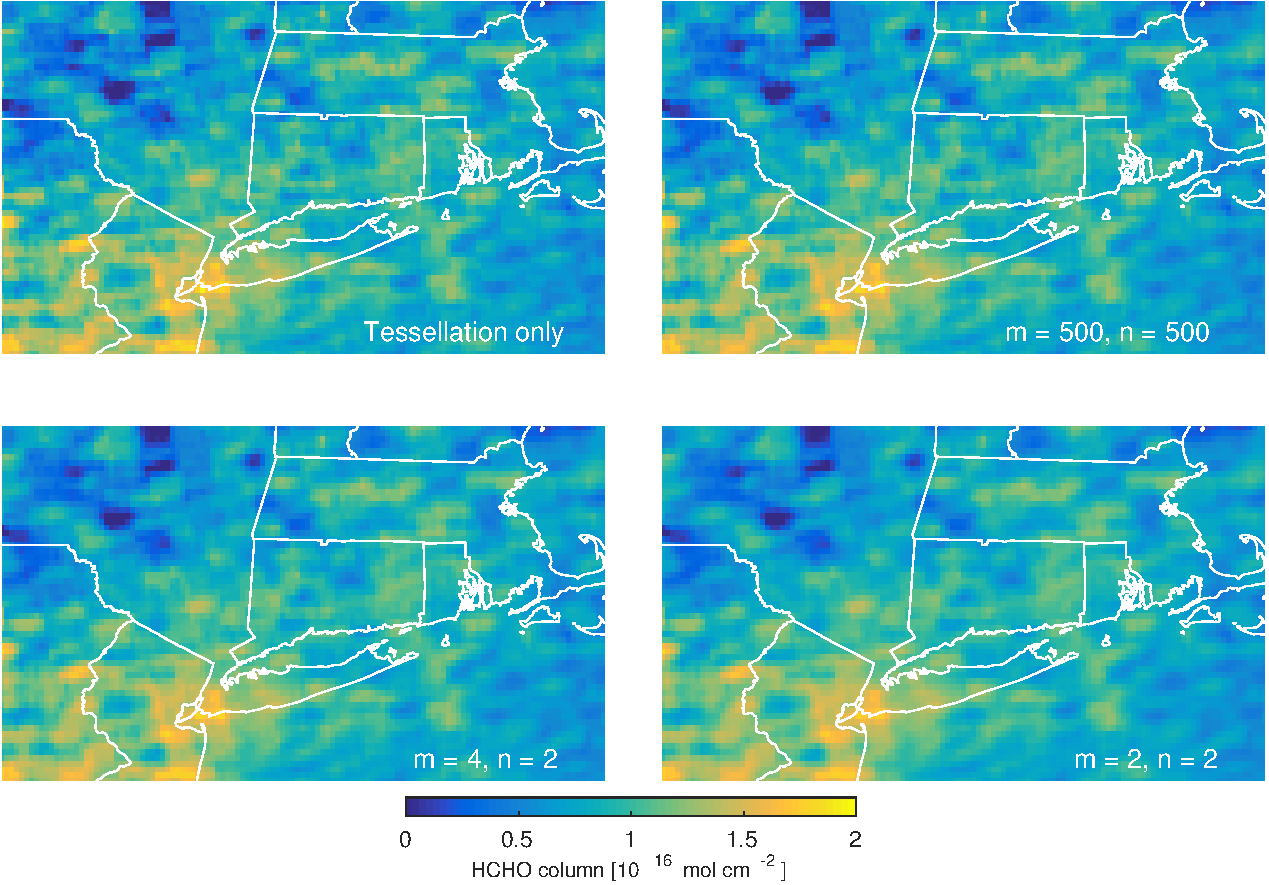
\includegraphics[width=.8\linewidth]{../plot/L3_compare.pdf}
 \caption{Oversampled HCHO map in the Northeast using OMI data in July 2005. Only cross-track positions 11--50 were included.}
 \label{fig6}
 \end{figure}
\section{Discussion}
\begin{enumerate}
\item The SRF does not have to be the physical OMI SRF. The exponents and even the FWHMs can be adjusted to include more spatial averaging and smoothing.
\item Current code is in Matlab. Eventually a Fortran version is necessary, which is much faster but much less flexible. 
\item Ideally the SRF should be defined on a plane normal to the radiance and on equal x-y space (instead of lat-lon). This may not be a big problem for OMI, as the distorted cross-track positions at large viewing angles have small weights anyway. But may worth consideration for TEMPO.
\end{enumerate}
\clearpage
\bibliographystyle{copernicus}
\bibliography{report_ref}

\end{document}


\section{Conclusions}
\begin{enumerate}
\item Super Gaussian is nice.
\item Linearizing the fitting using pseudo absorber is reasonably accurate if you know what you are doing.
\item Be careful with wavelength calibration using OMI preflight slit functions.
\end{enumerate}

\end{document}

